\newcommand{\psd}[1]{{\small\sffamily{\color{blue!60}#1}}}

In this section we present a 3D PSD simulation of a clamped bar which
his being loaded in vertical direction at the non-clamped end. This
simulation is like the one presented in previous tutorials, however in
3D. The material properties are same as before, and at the non-clamped
end traction \(t_y=-10^9\) units.The same problem from previous
tutorials 1 and 2 is used here in 3D, a bar 5 m in length and 1 m in
width and 1 m in height, and is supposed to be made up of a material
with density \(\rho=8\times 10^3\), Youngs modulus \(E=200\times 10^9\),
and Poissons ratio \(\nu=0.3\).

Here is how PSD simulation of this case can be performed.

\textbf{Step 1: Preprocessing}

First step in a PSD simulation is PSD preprocessing, at this step you
tell PSD what kind of physics, boundary conditions, approximations,
mesh, etc are you expecting to solve.

In the terminal \psd{cd} to the folder
\psd{/home/PSD-tutorials/linear-elasticity}. Launch
\psd{PSD\_PreProcess} from the terminal, to do so run the following
command.

\begin{lstlisting}[style=BashInputStyle]
PSD_PreProcess  -problem linear_elasticity -dimension 3 -dirichletconditions 1 -tractionconditions 1 -postprocess u
\end{lstlisting}

the comandline flag \psd{ -dirichletconditions 1} notifies to PSD that
there is one Dirichlet border ---the clamped end of the bar--- in this
simulation; \psd{ -dimension 3} means the simulation is 3D. And the flag
\psd{ -tractionconditions 1} notifies to PSD that there is one traction
border ---the right end of the bar--- in this simulation.

To provide Dirichlet conditions of the clamped end
(\(u_x=0,u_y=0,u_z=0\)) in \psd{ ControlParameters.edp} set
\psd{ Dbc0On 1}, \psd{ Dbc0Ux 0.}, \psd{ Dbc0Uy 0.}, and
\psd{ Dbc0Uz 0.}, where 1 being the surface mesh label of the clamped
end. To add the traction boundary condition set \psd{ Tbc0On 2} and
\psd{ Tbc0Ty -1.e9}, here the mesh label number of the right end is 2.
For this end \(\mathbf t=[t_x,t_y,t_z]=[0.,10^9,0.]\), hence in
\psd{ ControlParameters.edp} we only use \psd{ Tbc0Ty -1.e9}.

\textbf{Step 2: Solving}

Let us now use 4 cores to solve this problem. To do so enter the
following command:

\begin{lstlisting}[style=BashInputStyle]
PSD_Solve -np 4 Main.edp  -mesh ./../Meshes/3D/bar.msh -v 0
\end{lstlisting}

Notice, that this is the exact same command used in solving the previous
bar problems from other tutorials.

Note that for this simple problem, the bar mesh (\psd{bar.msh}) has been
provided in \psd{../Meshes/3D/"} folder, this mesh is a triangular mesh
produced with Gmsh. Moreover detailing meshing procedure is not the
propose of PSD tutorials. A user has the choice of performing their own
meshing step and providing them to PSD in
\psd{.msh}\footnote{Please use version 2} or \psd{.mesh} format, we
recommend using Salome or Gmsh meshers for creating your own geometry
and meshing them.

\textbf{Step 3: Postprocessing}

Launch ParaView and have a look at the \psd{ .pvd} file in the
\psd{ PSD/Solver/VTUs\_DATE\_TIME} folder.

\begin{figure}[htbp]
    \centering
    \begin{minipage}[t][2cm][t]{0.38\textwidth}
    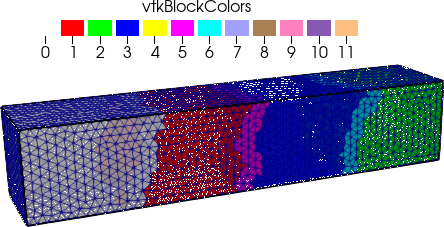
\includegraphics[align=b,width=1\textwidth]{./Images/3d-bar-clamped-ends.png}
    \end{minipage}\hspace{.1\textwidth}
    \begin{minipage}[t][2cm][t]{0.4\textwidth}
    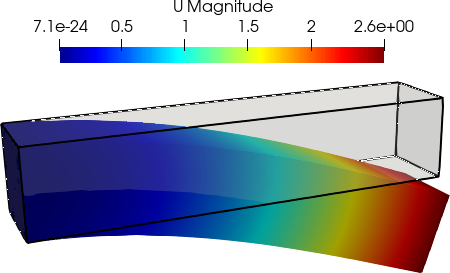
\includegraphics[align=b,width=1\textwidth]{./Images/3d-bar-clamped-pulled-partioned.png}
    \end{minipage}
    \caption{3D bar results. Partitioned mesh (left) and 0.5X warped displacement field (right).}
    \label{fig:3Dpart}
\end{figure}

In \cref{fig:3Dpart} there are four subdomais in the partitioned mesh
since four cores were used.
